\documentclass[12pt]{article}

\usepackage[margin = 1in]{geometry}
\usepackage{etex}
\usepackage{parskip, setspace}
\usepackage{amsfonts, amsmath, amssymb}
\usepackage{multirow, multicol}
\usepackage{epsfig}
\usepackage{placeins,graphicx}
\usepackage{verbatim, rotating, paralist}
\usepackage{caption, hanging}
\usepackage{pstricks, sgamevar, egameps}
\usepackage{lscape}
\usepackage{tikz}
\usepackage{hyperref}

% \usepackage{egamesps}
\usetikzlibrary{shapes, 
                arrows,
                backgrounds,
                decorations.pathmorphing,
                decorations.pathreplacing,
                calc,
                fadings,
                positioning}
% These are the key packages.  There is also sgame instead of sgamevar, but it doesn't work with beamer or other macros.
% The dcolumn package interferes with these, so you need to remove it from your preamble.

%Define your own tikz styles
\tikzstyle{startstop} = [rectangle, rounded corners, minimum width=1in, minimum height=0.5in,text centered, draw=black, fill=red!30]
\tikzstyle{dom} = [rectangle, rounded corners, minimum width=1in, minimum height=0.5in,text centered, draw=black, fill=red!30]
\tikzstyle{io} = [diamond, minimum width=0.25in, minimum height=2.3in, text centered, draw=black, fill=blue!30]
\tikzstyle{arrow} = [thick,->,>=stealth]
\tikzstyle{negarrow} = [thick,->,>=stealth, draw=red, fill=red]
\tikzstyle{assocarrow} = [thick,->,>=stealth, draw=green, fill=green]

%%%Everything below here is to give captions and legends
%to your custom diagrams
%Legend Code
\usepackage{pgfplots}
\newenvironment{customlegend}[1][]{%
    \begingroup
    % inits/clears the lists (which might be populated from previous
    % axes):
    \csname pgfplots@init@cleared@structures\endcsname
    \pgfplotsset{#1}%
}{%
    % draws the legend:
    \csname pgfplots@createlegend\endcsname
    \endgroup
}%

% makes \addlegendimage available (typically only available within an
% axis environment):
\def\addlegendimage{\csname pgfplots@addlegendimage\endcsname}

%%--------------------------------

% definition to insert numbers
\pgfkeys{/pgfplots/number in legend/.style={%
        /pgfplots/legend image code/.code={%
            \node at (0.125,-0.0225){#1}; % <= changed x value
        },%
    },
}
\pgfplotsset{
every legend to name picture/.style={west}
}

\usepackage{caption}
\captionsetup{font=scriptsize,labelfont=Large}

\title{Drawing Games and Diagrams in {\LaTeX} \footnote{This handout borrows heavily from previous handouts authored by Dave Ohls (2010) and 2013 materials from Richard Loeza.}}
\author{Sarah Bouchat (with additions by Michael Masterson)}
\date{September 19, 2018}

\begin{document}


\maketitle

This guide emphasizes a series of ways to draw game matrices and decision trees---both of which will be useful for 835 and 836---as well as providing some basic building blocks for drawing using {\LaTeX}. This should be considered a very rudimentary introductory guide---there are many more things to learn about drawing and figures in {\LaTeX} that are omitted here.\\


\section{Strategic Form Games}

Writing strategic form games using the \verb+sgamevar+ package creates diagrams that looks a lot like normal tabular environments, but it has the advantage of automatically tailoring the dimensions and labels to the alignment you want, rather than forcing you to do it by hand. There are a couple of things that distinguish it from a typical table environment:

\begin{compactitem}
\item Use the ``figure'' float instead of the ``table'' float.
\item The \verb+\>+ replaces \verb+&+ as the divider between cells. Note that in the \verb+sgame+ package, you use \verb+&+ still. 
\item The initial operators are different: rather than \verb+\begin{tabular}{l|cc}...\end{tabular}+ it is: \\ 
\small 
\verb+\begin{game}{rows}{columns}[player 1 label][player 2 label][figure label]...\end{game}+ \\
\end{compactitem}

\begin{figure}[h!]
\begin{center}
\begin{footnotesize}
\begin{game}{2}{3}[1][2][]
        \> Left \> Center \> Right   \\
Top      \> 3,2  \> 4,4    \> 2,1   \\
Bottom    \> 1,1  \> 5,7    \> 4, 3 \\
\end{game}
\end{footnotesize}
\end{center}
\end{figure}

Most stylistic commands also work inside games. Using circles to indicate best responses is problematic because the circles tend to cut off some of the numbers. You can also use highlighting.

\begin{figure}[h!]
\begin{footnotesize}
 \begin{center}
\begin{game}{5}{5}[\textbf{1}][\textbf{2}][Ammunition]
       \> Rock    \> Paper   \> Scissors \> Flamethrower \> Water Canon  \\
Rock \> \underline{1,1}  \>  0,2  \> 2,0 \> 2,0 \> 0,2 \\
 Paper \> 2,0    \> \underline{1,1}  \> 0,2 \> 0,2 \> 2,0 \\
 Scissors \> 0,2 \> 2,0 \> \underline{1,1} \> 2,0 \> 0,2 \\
Flamethrower \> 0,2  \> 2,0 \> 0,2 \> \underline{1,1} \> 2,0 \\
 Water Canon \> 2,0 \> 0,2 \> 2,0 \> 0,2 \> \textcircled{1},\textcircled{1} \\
\end{game}
\end{center}
\end{footnotesize}
\end{figure}

\sgcolsep=0.5pt
\renewcommand{\gamestretch}{1.5}
\def\highlight#1{\colorbox{lightgray}{#1}}
\fboxsep=5pt
\begin{figure}[htb]\hspace*{\fill}%
\begin{center}
\begin{game}{3}{3}[{\em Bob}     ][{\em Jim}][]
        \> A \> B \> C   \\
X \>8,6\> 6,8 \> 0,0   \\
Y \> 6,8  \> 8,6 \> 0,0 \\
Z \> 0,0 \> 0,0 \>\highlight{5,5}\\
\end{game} 
\end{center} 
\end{figure}
 
\FloatBarrier
\section{Extensive Form Games}
Previous versions of this workshop used the \verb+egamesps+ package to create extensive form games. That package makes creating extensive games simpler, but it is very prone to errors and much less flexible than using the tikz approach. Be aware that using egamesps may require you to use a different compilation engine for your {\LaTeX} document (e.g., XeTeX).

% \begin{figure}[htb]
% \hspace*{\fill}
% \begin{egame}(600,280)
% \putbranch(300,240)(2,1){200}
% \iib{1}{$C_a$}{$D_a$}
% \putbranch(100,140)(1,1){100}
% \egalhshift=20
% \iib{$2_a$}{$C$}{$D$}[$2,2$][$0,3$]
% \putbranch(500,140)(1,1){100}
% \egalhshift=20
% \iib{$2_b$}{$C$}{$D$}[$3,0$][$1,1$]
% \end{egame}
% \hspace*{\fill}
% \caption[]{Sequential PD}
% \end{figure}

Instead of dealing with these issues, you can create extensive form games using the \verb+tikzpicture+ environment, from the tikz package. The tikz package is designed for drawing in general, and is very flexible. The package can accommodate nearly any shape or arrangement you desire. The basic syntax of the coding language involves drawing a series of objects (lines, geometric shapes, text), specifying their location on a coordinate scale, and specifying the properties you want them to have (size, style, color, shading, special features). 


\begin{center}
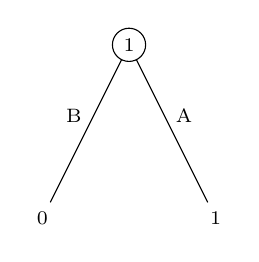
\begin{tikzpicture}[scale=1]
\draw(0,2) -- (1,0);
\draw(0,2) -- (-1,0);
\draw (.7,1.1) node{\scriptsize{A}};
\draw (-.7,1.1) node{\scriptsize{B}};
\draw(1.1,-.2) node {\scriptsize{1}};
\draw(-1.1,-.2) node {\scriptsize{0}};
\filldraw[fill=white](0,2) circle (6pt) node{\scriptsize{1}};
\end{tikzpicture}
\end{center}

What the commands are doing: \\

\begin{compactitem}
\item \verb+[scale=1]+Scales the figure with the dimensions given (in centimeters).  Increase (or decrease) the scale to expand (or shrink) the figure.
\item \verb+\draw (0,2) -- (1,0);+: Draws a straight line between coordinate points (0,2) and (1,0).
\item \verb+\draw (.7,1.1) node{\scriptsize{A}};+ Creates a node with the small text A at the coordinates (.7,1.1).
\item \verb+\filldraw[fill=white](0,2) circle (6pt) node{\scriptsize{1}};+ Creates a circle, 6 points in diameter and fills the inside white. It then creates a small 1 in the middle of the circle. Note that this will cover up anything under the filled circle. 
\end{compactitem}
\vspace{.5cm}
With tikz, the order in which objects are rendered is important. A filled circle will go over anything at the same coordinates if it is listed after those things. Note how the above figure looks when the ordering is changed.

\begin{center}
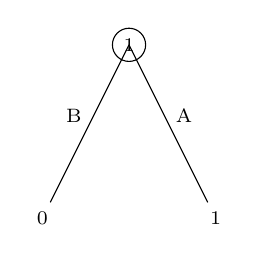
\begin{tikzpicture}[scale=1]
\filldraw[fill=white](0,2) circle (6pt) node{\scriptsize{1}};
\draw(0,2) -- (1,0);
\draw(0,2) -- (-1,0);
\draw (.7,1.1) node{\scriptsize{A}};
\draw (-.7,1.1) node{\scriptsize{B}};
\draw(1.1,-.2) node {\scriptsize{1}};
\draw(-1.1,-.2) node {\scriptsize{0}};
\end{tikzpicture}
\end{center}

Note that every line in a tikzpicture ends in a semicolon. A common error is forgetting to put one in.\\

With these basic tools, you can make games in a variety of shapes.

\begin{center}
\begin{scriptsize}
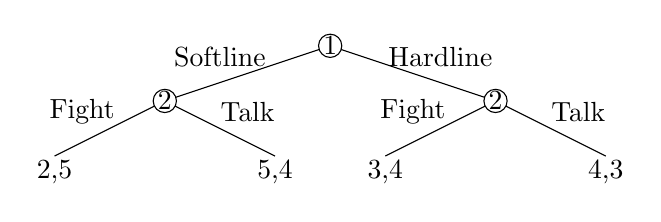
\begin{tikzpicture}[scale=.7]
\draw(7,3) -- (4,2);
\draw(7,3) -- (10,2);
\draw (5,2.8) node{Softline};
\draw (9,2.8) node{Hardline};
\draw(4,2) -- (2,1);
\draw(4,2) -- (6,1);
\draw (2.5,1.8) node{Fight};
\draw (5.5,1.8) node{Talk};
\draw(10,2) -- (8,1);
\draw(10,2) -- (12,1);
\draw (8.5,1.8) node{Fight};
\draw (11.5,1.8) node{Talk};
\filldraw[fill=white](7,3) circle (6pt) node{1};
\filldraw[fill=white](4,2) circle (6pt) node{2};
\filldraw[fill=white](10,2) circle (6pt) node{2};
\draw(2,.7) node {2,5};
\draw(6,.7) node {5,4};
\draw(8,.7) node {3,4};
\draw(12,.7) node {4,3};
\end{tikzpicture}
\end{scriptsize}
\end{center}

\begin{center}
\begin{footnotesize}
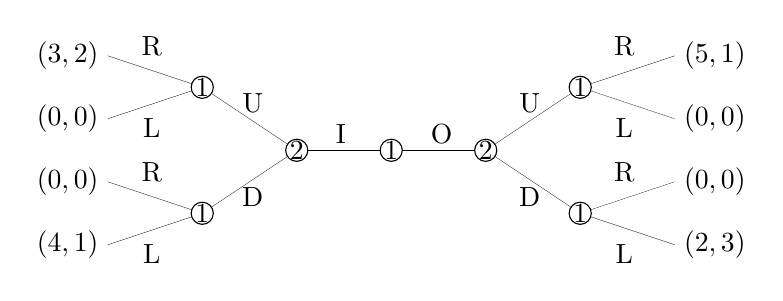
\begin{tikzpicture}[scale=.8]
\draw[ultra thin] (6,0) -- (7.5,1); 
\draw[ultra thin] (6,0) -- (7.5,-1);
\draw[ultra thin] (6,0) -- (4.5,0);
\draw[ultra thin] (3,0) -- (4.5,0);
\draw[ultra thin] (3,0) -- (1.5,1); 
\draw[ultra thin] (3,0) -- (1.5,-1);
\draw (6.7,.75) node{U};
\draw (6.7,-.75) node{D};
\draw (2.3,.75) node{U};
\draw (2.3,-.75) node{D};
\draw (3.7,.25) node{I};
\draw (5.3,.25) node{O};
\filldraw[fill=white] (6,0) circle (5pt) node {2};
\filldraw[fill=white] (3,0) circle (5pt) node {2};
\filldraw[fill=white] (4.5,0) circle (5pt) node {1};
\draw[ultra thin] (7.5,-1) -- (9,-.5) node[right]{$(0,0)$};
\draw[ultra thin] (7.5,-1) -- (9,-1.5) node[right]{$(2,3)$};
\draw (8.2,-.35) node{R};
\draw (8.2,-1.65) node{L};
\draw (8.2,.35) node{L};
\draw (8.2,1.65) node{R};
\filldraw[fill=white] (7.5,-1) circle (5pt) node {1};
\draw[ultra thin] (7.5,1) -- (9,.5) node[right]{$(0,0)$};
\draw[ultra thin] (7.5,1) -- (9,1.5) node[right]{$(5,1)$};
\filldraw[fill=white] (7.5,1) circle (5pt) node {1};
\draw[ultra thin] (1.5,1) -- (0,.5) node[left]{$(0,0)$};
\draw[ultra thin] (1.5,1) -- (0,1.5) node[left]{$(3,2)$};
\draw[ultra thin] (1.5,-1) -- (0,-.5) node[left]{$(0,0)$};
\draw[ultra thin] (1.5,-1) -- (0,-1.5) node[left]{$(4,1)$};
\draw (.7,-.35) node{R};
\draw (.7,-1.65) node{L};
\draw (.7,.35) node{L};
\draw (.7,1.65) node{R};
\filldraw[fill=white] (1.5,1) circle (5pt) node {1};
\filldraw[fill=white] (1.5,-1) circle (5pt) node {1};
\end{tikzpicture}
\end{footnotesize}
\end{center}

\section{Make Custom Diagrams with Tikz}
You can make your own custom diagrams with Tikz. Often these are used to make diagrams of causal processes, but you could potentially use it for anything.

\subsection{Defining Custom Shapes}
First you need to define the shapes you wil use in the preamble. In this document's preamble I define the shapes as follows:
\begin{tiny}
\begin{verbatim}
\tikzstyle{startstop} = [rectangle, rounded corners, minimum width=1in, minimum height=0.5in,text centered, draw=black, fill=red!30]
\tikzstyle{dom} = [rectangle, rounded corners, minimum width=1in, minimum height=0.5in,text centered, draw=black, fill=red!30]
\tikzstyle{io} = [diamond, minimum width=0.25in, minimum height=2.3in, text centered, draw=black, fill=blue!30]
\tikzstyle{arrow} = [thick,->,>=stealth]
\tikzstyle{negarrow} = [thick,->,>=stealth, draw=red, fill=red]
\tikzstyle{assocarrow} = [thick,->,>=stealth, draw=green, fill=green]
\end{verbatim} 
\end{tiny}
The bracers {} after `\textbackslash{tikzstyle}' define the name of the shape. In the square brackets, the shape of the shape, its size, color, and orientation can be defined.
\FloatBarrier

\subsection{Making Diagrams}

Figure \ref{dside} shows the causal process of the dark side according to Yoda using only the startstop shape and the arrow shape.

\begin{centering}
\begin{figure} 
	\caption{\Large The Darkside Causal Process Diagram}
		\label{dside}
        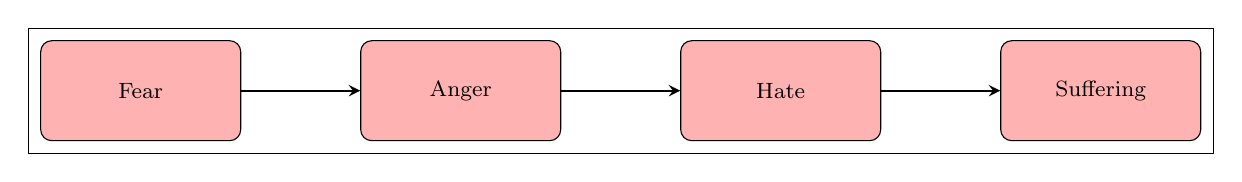
\begin{tikzpicture}[framed, node distance=1.6in]
        \begin{footnotesize}
        	\node (start) [startstop, anchor = west] {Fear};
			\node (anger) [startstop, right of=start] {Anger};
			\node (hate) [startstop, right of = anger] {Hate};
			\node (suffering) [startstop, right of=hate] {Suffering};
			\draw [arrow] (start) --  (anger);
			\draw [arrow] (anger) -- (hate);
			\draw [arrow] (hate) -- (suffering);
			% 
        \end{footnotesize}
        \end{tikzpicture}
\end{figure}
\end{centering}

\FloatBarrier
Here is the code used to make Figure \ref{dside}:
\begin{verbatim}
\begin{centering}
\begin{figure} 
	\caption{\Large The Darkside Causal Process Diagram}
		\label{dside}
        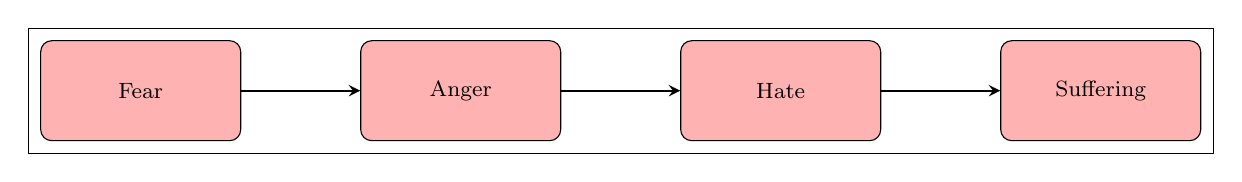
\begin{tikzpicture}[framed, node distance=1.6in]
        \begin{footnotesize}
        	\node (start) [startstop, anchor = west] {Fear};
			\node (anger) [startstop, right of=start] {Anger};
			\node (hate) [startstop, right of = anger] {Hate};
			\node (suffering) [startstop, right of=hate] {Suffering};
			\draw [arrow] (start) --  (anger);
			\draw [arrow] (anger) -- (hate);
			\draw [arrow] (hate) -- (suffering);
			% 
        \end{footnotesize}
        \end{tikzpicture}
\end{figure}
\end{centering}
\end{verbatim}
In the call to tikzpicture, I define the distance between nodes as well as whether the picture is framed. To create a node, use \textbackslash{node} and follow it with its name. In the square brackets, specify the name of the node you defined in the preamble that you wish to use as well as the relative location of the node. You can add text to the node inside bracers at the end of the line.

You can also add text above arrows, use multiple shapes in a single diagram, and create a legend. See figure 2 below:


\begin{figure} \label{theory}
\caption{\Large Theorized Relationships}
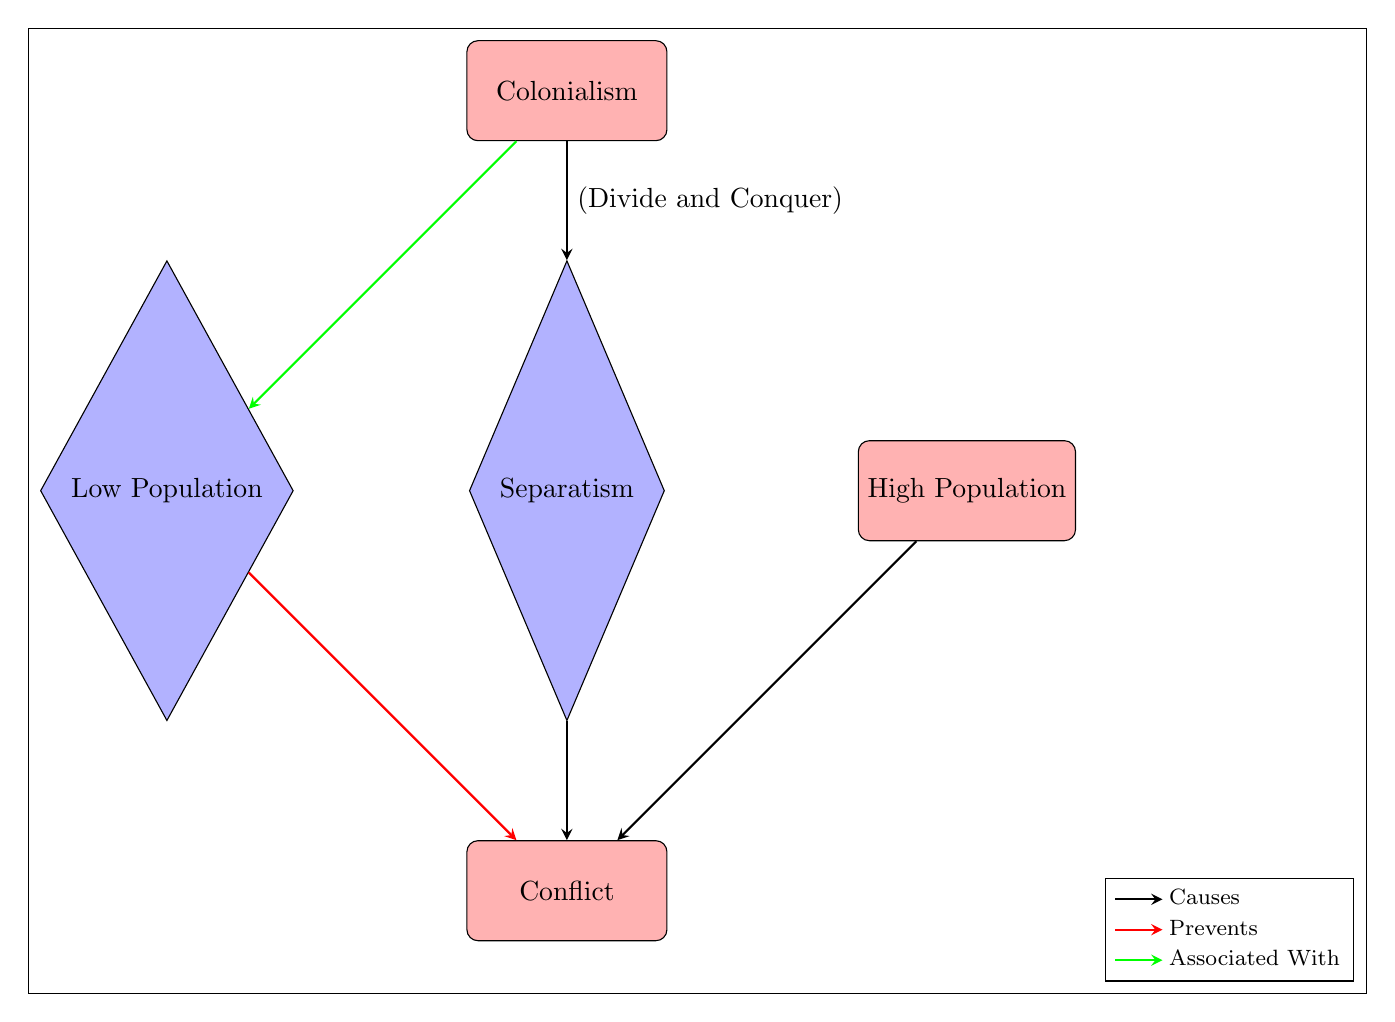
\begin{tikzpicture}[framed, node distance=2in] 
\node (start) [startstop] {Colonialism};
\node (in2) [io, below of=start] {Separatism};
\node (in1) [io, left of=in2] {Low Population};
\node (start2) [startstop, right of =in2] {High Population};
\node (stop) [startstop, below of=in2] {Conflict};
\draw [arrow] (start) --node[right] {(Divide  and Conquer)} (in2);
\draw [arrow] (in2) -- (stop);
\draw [assocarrow] (start) -- (in1);
\draw [negarrow] (in1) -- (stop);
\draw [arrow] (start2) -- (stop);
\begin{customlegend}[legend cell align=left,
legend entries={
Causes,
Prevents,
Associated With,
},
legend style={at={(10,-10)},font=\footnotesize}] % <= to define position and font legend
% the following are the "images" and numbers in the legend
	\addlegendimage{arrow}
	\addlegendimage{negarrow}
	\addlegendimage{assocarrow}
\end{customlegend}

\end{tikzpicture}
\end{figure}
\FloatBarrier

To add text next to an arrow just add `node[relative location]' and {text you want to add} after the 
\begin{verbatim}`--'\end{verbatim}
and before the second shape the arrow connects with. For example: \begin{verbatim}
\draw [arrow] (start) --node[right] {(Divide  and Conquer)} (in2);
\end{verbatim}

To add a legend, add a list of legend entries that you want to be the labels of the legend, specify the size and font of the legend, and lastly add the tikz shaped you want the legend to label. The legend should be within the tikz picture environment. The code to make the legend in 
Figure 2 is the following:
\begin{verbatim}
\begin{customlegend}[legend cell align=left,
legend entries={
Causes,
Prevents,
Associated With,
},
legend style={at={(10,-10)},font=\footnotesize}] % <= to define position and font legend
% the following are the "images" and numbers in the legend
	\addlegendimage{arrow}
	\addlegendimage{negarrow}
	\addlegendimage{assocarrow}
\end{customlegend}
\end{verbatim}

\end{document}
